\section{Evaluation}

We first look at results found using our assembly micro-benchmark on x86\_64.  
We then look at other architectures to see if the same limitations apply.  
We analyze methods for mitigating the variations in counts.  
Finally we attempt to apply our methodology to a full benchmark suite.

\subsection{Sources of Overcount and Non-Determinism on x86\_64}

\label{details}

We use our hand-crafted assembly language benchmark
to find deviation from the known expected count.  
We are interested in {\em nondeterminism}
(run-to-run variations) and {\em overcount}
(always-the-same predictable offsets against known event count 
due to errata in the chip design).

We calculate known total event counts for the various metrics
via code inspection, and then validate the expected counts with the 
Pin~\cite{luk+:pldi05} dynamic binary instrumentation (DBI) tool.
We use a script to gather performance counter totals for each platform;
in the common case where counter results do not match expectations we
manually comment out parts of the assembly benchmark and re-run
until we localize the source of variation.  

% Determinism Table

\begin{table*}[tbp]
\caption{Summary of sources of nondeterminism and overcount for
         retired instructions.}
\label{table:deterministic_events}
\centering
\begin{tabular}{|l||c|c|c|c|c|c|}

\hline
            	&
Total		&
Total		&
Conditional	&
\multirow{2}{*}{Loads}			&
\multirow{2}{*}{Stores}			\\


	&
Instructions	&
Branches	&
Branches	&
	&
	\\


\hline
\hline


%%%%%%%%%%%%%%%%%%%%%%
% Atom
%%%%%%%%%%%%%%%%%%%%%%
Atom	& 
hpEF	& % Total Instructions
hp	& % Total Branches
--	& % Conditional Branches
--	& % Retired Loads 
--	\\ % Retired Stores
\hline

%%%%%%%%%%%%%%%%%%%%%%
% Core2
%%%%%%%%%%%%%%%%%%%%%%
Core2	&
hpEF	& % Total Instructions
hpD	& % Total Branches
p	& % Conditional Branches
hpD	& % Retired Loads
{\scriptsize \bf DETERMINISTIC}	\\ % Retired Stores
\hline

%%%%%%%%%%%%%%%%%%%%%%
% Nehalem
%%%%%%%%%%%%%%%%%%%%%%
Nehalem &
hpEF	& % Total Instructions
hp	& % Total Branches
D	& % Conditional Branches
hpM	& % Retired Loads
hpD	\\ % Retired Stores
\hline

%%%%%%%%%%%%%%%%%%%%%%
% Westmere
%%%%%%%%%%%%%%%%%%%%%%
Westmere	&
hpEF	& % Total Instructions
hp	& % Total Branches
{\scriptsize \bf DETERMINISTIC}	& % Conditional Branches
hp	& % Retired Loads
hpD	\\ % Retired Stores
\hline

%%%%%%%%%%%%%%%%%%%%%%
% SNB/IVB/HSW
%%%%%%%%%%%%%%%%%%%%%%
Sandybridge		&
\multirow{3}{*}{hpEF}	& % Total Instructions
\multirow{3}{*}{hp}	& % Total Branches
\multirow{3}{*}{\scriptsize \bf DETERMINISTIC}	& % Conditional Branches
\multirow{3}{*}{U}	& % Retired Loads
\multirow{3}{*}{U}	\\ % Retired Stores

IvyBridge		&
			& % Total Instructions
			& % Total Branches
			& % Conditional Branches
			& % Retired Loads
			\\ % Retired Stores

Haswell			&
			& % Total Instructions
			& % Total Branches
			& % Conditional Branches
			& % Retired Loads
			\\ % Retired Stores
\hline

%%%%%%%%%%%%%%%%%%%%%%
% Pentium D
%%%%%%%%%%%%%%%%%%%%%%
Pentium D	&
hpEFD		& % Total Instructions
hp		& % Total Branches
!		& % Conditional Branches
hpU		& % Retired Loads
hpU		\\ % Retired Stores
\hline

%%%%%%%%%%%%%%%%%%%%%%%%%
% Phenom/Instanbul/Bobcat
%%%%%%%%%%%%%%%%%%%%%%%%%
Phenom		&
\multirow{3}{*}{hpEFD}	& % Total Instructions
\multirow{3}{*}{hp}	& % Total Branches
\multirow{3}{*}{--}	& % Conditional Branches
\multirow{3}{*}{--} 	& % Retired Loads
\multirow{3}{*}{--}	\\ % Retired Stores

Istanbul		&
			& % Total Instructions
			& % Total Branches
			& % Conditional Branches
			& % Retired Loads
			\\ % Retired Stores

Bobcat			&
			& % Total Instructions
			& % Total Branches
			& % Conditional Branches
			& % Retired Loads
			\\ % Retired Stores
\hline

\end{tabular}



\vspace{2ex}
\begin{tabular}{|l|c|l|}
\hline
Sources of nondeterminism: & {\bf h} & Hardware Interrupts \\
                           & {\bf p} & Page Faults \\
\hline
Sources of overcount:       & {\bf E} & x87/SSE exceptions \\
                           & {\bf F} & OS Lazy FP handling \\
                           & {\bf D} & Instructions Overcounted \\
                           & {\bf M} & Instructions Undercounted \\
                           & {\bf U} & Counts micro-ops \\
\hline
Missing Results:           & {\bf --} & Event not available \\
                           & {\bf !}  & Test not run \\
\hline
\end{tabular}
\end{table*}

% uop table

\begin{table*}[tbp]
\caption{Retired $\mu$ops, multiplies, and divides 
         in the microbenchmark;  these values vary from machine 
         to machine.}
\label{table:results_uops}

\centering
%\begin{table*}[tbp]
%\tbl{Retired $\mu$ops, multiplies, and divides in the microbenchmark.
%These values vary greatly from machine to machine.}
%\caption{Retired $\mu$ops, multiplies, and divides in the microbenchmark.
%These values vary greatly from machine to machine.
%\label{table:results_uops}
%}
%{
%\sffamily
%\begin{center}
\begin{tabular}{|l||r@{$\pm$}r||r@{$\pm$}r||r@{$\pm$}r|}

\hline
Machine   & \multicolumn{2}{c||}{$\mu$ops} & \multicolumn{2}{c||}{Multiplies} & \multicolumn{2}{c|}{Divides} \\

\hline
\hline

Atom           & 12,650,929,921 & 10,048 &  13,700,000 &  0     &   7,000,000 & 0      \\
\hline
Core2          & 14,250,314,285 & 38,796 &  16,300,012 & 13     &   5,800,058 & 16 \\
\hline
Nehalem        & 11,746,800,094 & 38,192 & 17,719,572 & 1,992,446 & 3,180,368 & 7,409    \\
\hline
Nehalem-EX     & 11,746,938,597 & 27,708 & 19,835,890 & 215,301   &  3,265,181 & 21,966    \\
\hline
Westmere-EX       & 11,740,683,274 & 218,900 & 19,866,413 & 196,031 & 5,800,072           &  64 \\
\hline
SandyBridge-EP  & 12,292,221,237 &  7,258 & \multicolumn{2}{c||}{n/a}   &  5,800,304 & 56    \\
\hline
IvyBridge      & 12,315,297,486 & 4,669,700 & 620,550    & 17,451           &  3,244,139          & 17,414 \\
\hline
Haswell		& 12,128,839,684 & 4684 & 600,024 & 6 & \multicolumn{2}{c||}{n/a} \\
\hline
Pentium D      & 12,555,222,761 & 6,650,825 & \multicolumn{2}{c||}{n/a} & \multicolumn{2}{c|}{n/a} \\
\hline
Phenom         & 10,550,974,722 & 36,819 &  69,242,930 & 62,492  & \multicolumn{2}{c|}{n/a} \\
\hline
Istanbul       & 10,557,954,252 & 168,608 &  69,988,147 & 317,885    & \multicolumn{2}{c|}{n/a} \\
\hline
Fam14h         & 11,366,903,273 & 153,234   &   1,800,000 & 0    & 2,400,000 & 0 \\
\hline
\end{tabular}
%\end{center}
%}
%
%\end{table*}


\end{table*}

% FP table

\begin{table*}[tbp]

\caption{Retired FP, MMX and SSE instructions in the microbenchmark.
        These values vary from machine to machine.  
        Some may be
        deterministic, but cannot be used with integer-only 
        workloads.}
\label{table:results_fp}

\centering
%\begin{table*}[tbp]
%\caption{Retired FP, MMX and SSE instructions in the microbenchmark.
%These values also vary from machine to machine.  Some of these
%are deterministic, but cannot be used when analyzing integer-only workloads.
%\label{table:results_fp}
%}

%\tbl{Retired FP, MMX and SSE instructions in the microbenchmark.
%These values also vary from machine to machine.  Some of these
%are deterministic, but cannot be used when analyzing integer-only workloads.}
%{
%\sffamily
%\begin{center}
\begin{tabular}{|l||r@{$\pm$}r|r@{$\pm$}r|r@{$\pm$}r|}

\hline
Machine   & 
\multicolumn{2}{c|}{FP1} & 
\multicolumn{2}{c|}{FP2} & 
\multicolumn{2}{c|}{SSE} \\
\hline
\hline

Atom         &  38,800,000 &   0 & 44,000,221 & 341 & 88,293,855 & 70,345 \\
\hline
Core2        &  72,601,258 & 215 &  39,099,997 & 0 & 23,200,000 & 0   \\
\hline
Nehalem      &  50,234,437 & 6,800 &  17,199,998 & 2 & 24,203,034 & 563 \\
\hline
Nehalem-EX   &  50,230,521 & 5,827 &  17,199,998 & 4 & 24,028,996 & 222,406 \\
\hline
Westmere-EX  &  50,015,343 & 43,898 & 17,199,998 & 2  & 24,921,548 & 38,051 \\
\hline
SandyBridge-EP &  48,784,041 & 1,325 &  17,200,028 & 8 & 23,136,313 & 18,585 \\
\hline
IvyBridge    &  49,025,110 & 37,400 & 17,200,040 & 27 &  5,434,935 & 26,195  \\
\hline
Haswell		& \multicolumn{2}{c|}{n/a} & \multicolumn{2}{c|}{n/a} & \multicolumn{2}{c|}{n/a} \\
\hline
Pentium D    & 100,400,310 & 413 & \multicolumn{2}{c|}{n/a} & 28,795,097 & 5,662\\
\hline
Phenom       & 26,600,001 & 0  & 112,700,001 & 0 &  15,800,000 & 0\\
\hline
Istanbul     & 26,600,001 & 0  & 112,700,001 & 0 & 15,800,000 & 0 \\
\hline
Fam14h       & 115,199,563 & 21  & 276,217,480 & 541,728 & 15,800,000 & 0 \\
\hline
\end{tabular}
%\end{center}
%}
%
%\end{table*}


\end{table*}


Table~\ref{table:deterministic_events} shows a summary of the overcount
and nondeterminism found on each system.  The actual event totals
gathered are not important; they are arbitrary values related to
the instruction mix of the benchmark.  They key below the table
describes the sources of variation, as described below.

\subsubsection{Nondeterministic Hardware Interrupts}

Most x86\_64 events are incremented an extra time for every hardware 
interrupt that occurs (the most common hardware interrupt is the 
periodic timer, causing a noticeable runtime-related variation).
This interrupt behavior was originally undocumented when we first
described it, but now appears in some vendor documentation.  
The number of extra events is inherently unpredictable,
but often can be measured with an additional ``hardware interrupts''
event that can be used to adjust the total aggregate results.  
If an event is affected by hardware interrupts, then it cannot be a 
deterministic event, as it is impossible to predict in advance when
these events will happen.

Another source of interrupts is generated
when a page fault occurs; in general
the first time a page of memory is accessed it causes a page fault 
that counts as an extra instruction.  This variation is more predictable
than other interrupts, but can still be affected by the behavior of
the operating system and other programs running on the system.


\subsubsection{Sources of Instruction Overcount}

There are various sources that can cause overcount on x86 processors.

On all the systems we tested an extra instruction event happens if the 
x87 top-of-stack pointer overflows; care is taken in our benchmark to 
avoid this condition.  

An additional count may happen when the floating point unit is 
used for the first time; this is due to
the lazy floating-point save mechanism used by Linux to avoid context-switch 
overhead for non-floating point applications.  

A major source of overcount is when an instruction event is incremented
multiple times for a single instruction, or when an instruction
is not counted at all.  This is likely due to missing terms in the
instruction classifying hardware on the PMU.

One last source of overcount is when an event measures microcoded events
rather than retired events.  Sometimes these events are deterministic,
but it is hard to verify because microcode is system dependent and
undocumented.  Recent counter documentation has gotten much better
at indicating which events are architectural instructions and which 
are microcoded.

\paragraph {Total Retired Instruction Overcount}

The total retired instructions event is high-profile and often used,
but still may be affected by overcount.

While not strictly a source of overcount, some instructions are
actually pseudo-instructions and can confuse a user 
determining expected instruction counts
via code inspection.
Various x87 floating point instructions have ``wait'' and ``no wait''
versions that optionally force execution to wait to see if an exception
has occurred.  
The wait versions are pseudo-ops for instructions with a wait prefix
and count twice.

The AMD machines overcount by one when
{\tt fninit}, {\tt fnsave}, and {\tt fnclex} instructions execute
and one of the FP exception status word flags (such as PE or ZE) is set.
Despite being interrupt related, this variation
is an overcount because it can be predicted and happens deterministically.

The Pentium~D processor has two different 
retired instruction events.  
The newer (not available on earlier Pentium~4 models)
event is {\tt INSTRUCTIONS\_COMPLETED:NBOGUS} which behaves like the 
corresponding event on other processors.
The other event, {\tt INSTRUCTIONS\-\_RETIRED\-:NBOGUSNTAG} is very different.
It is not affected by hardware interrupts (unless those interrupts cause a 
string instruction to re-start).  
This has the potential to be a deterministic event; however 
it suffers from overcount with the following instructions:
{\tt fldcw}, 
{\tt fldenv}, {\tt frstor}, {\tt maskmovq}, {\tt emms}, {\tt cvtpd2pi} (mem),
{\tt cvttpd2pi} (mem), {\tt sfence}, and {\tt mfence}.  
The {\tt fldcw}
instruction is particularly troublesome as it is a common instruction
used when converting floating point values to integers (and it has
been shown to cause up to 2\%
overcount on some SPEC CPU benchmarks~\cite{weaver+:iiswc08}).

\paragraph{Retired Branches Overcount}
The retired branches event counts control flow changes, 
including system call entry.

On AMD processors, the perf\_event {\tt branches:u} generalized event counts 
the wrong value.  We supplied a fix that was incorporated into the 2.6.35
kernel; care must be taken to use the proper 
raw event on earlier kernels.

On Core2 processors the {\tt cpuid} instruction also counts as a branch.

\paragraph{Retired Conditional Branches Overcount}
Not all processors support counting 
conditional branches (and we were unable
to test on Pentium~D as the machine we used 
for the other results has been decommissioned).

Noll~\cite{noll:pc2011} reports that this event
is deterministic on SandyBridge; we have verified
this result and found that the equivalent event
is likewise deterministic on Westmere and Nehalem.
The Nehalem event suffers from overcount:
in addition to conditional branches (which start with opcode {\tt 0F})
many instructions are counted that also start with opcode {\tt 0F},
including various non-branch MMX and SSE instructions.

\subsubsection{Retired Load Overcount} 
Retired loads are not supported on all of the processors we investigate.
Extra loads are counted on exceptions: first floating point usage,
page faults, x87 FPU exceptions and SSE exceptions.

Load events are subject to various forms of under and overcount.
Conditional move instructions will {\em always} register a 
load from memory, even if the condition is not met.
The {\tt fbstp} ``store 80-bit BCD'' instruction counts as
a load.  The {\tt cmps} string compare instruction (where two values from 
distinct memory are loaded and then compared) counts as only being
a single load.

On Core2 machines the {\tt leave} instruction counts as two loads.
The {\tt fstenv}, {\tt fxsave},  and {\tt fsave} floating point
state-save instructions also count as loads.
The  {\tt maskmovq} and  {\tt maskmovdqu} count loads even though
they only write to memory.  The {\tt movups}, {\tt movupd} and 
{\tt movdqu} instructions count as loads even if their operands
indicate a store-to-memory operation.

On Nehalem processors the {\tt paddb}, {\tt paddw}, and {\tt paddd}
do {\em not} count as load operations even if the their operands
indicate a load from memory.

\begin{figure}[!t]
\centering
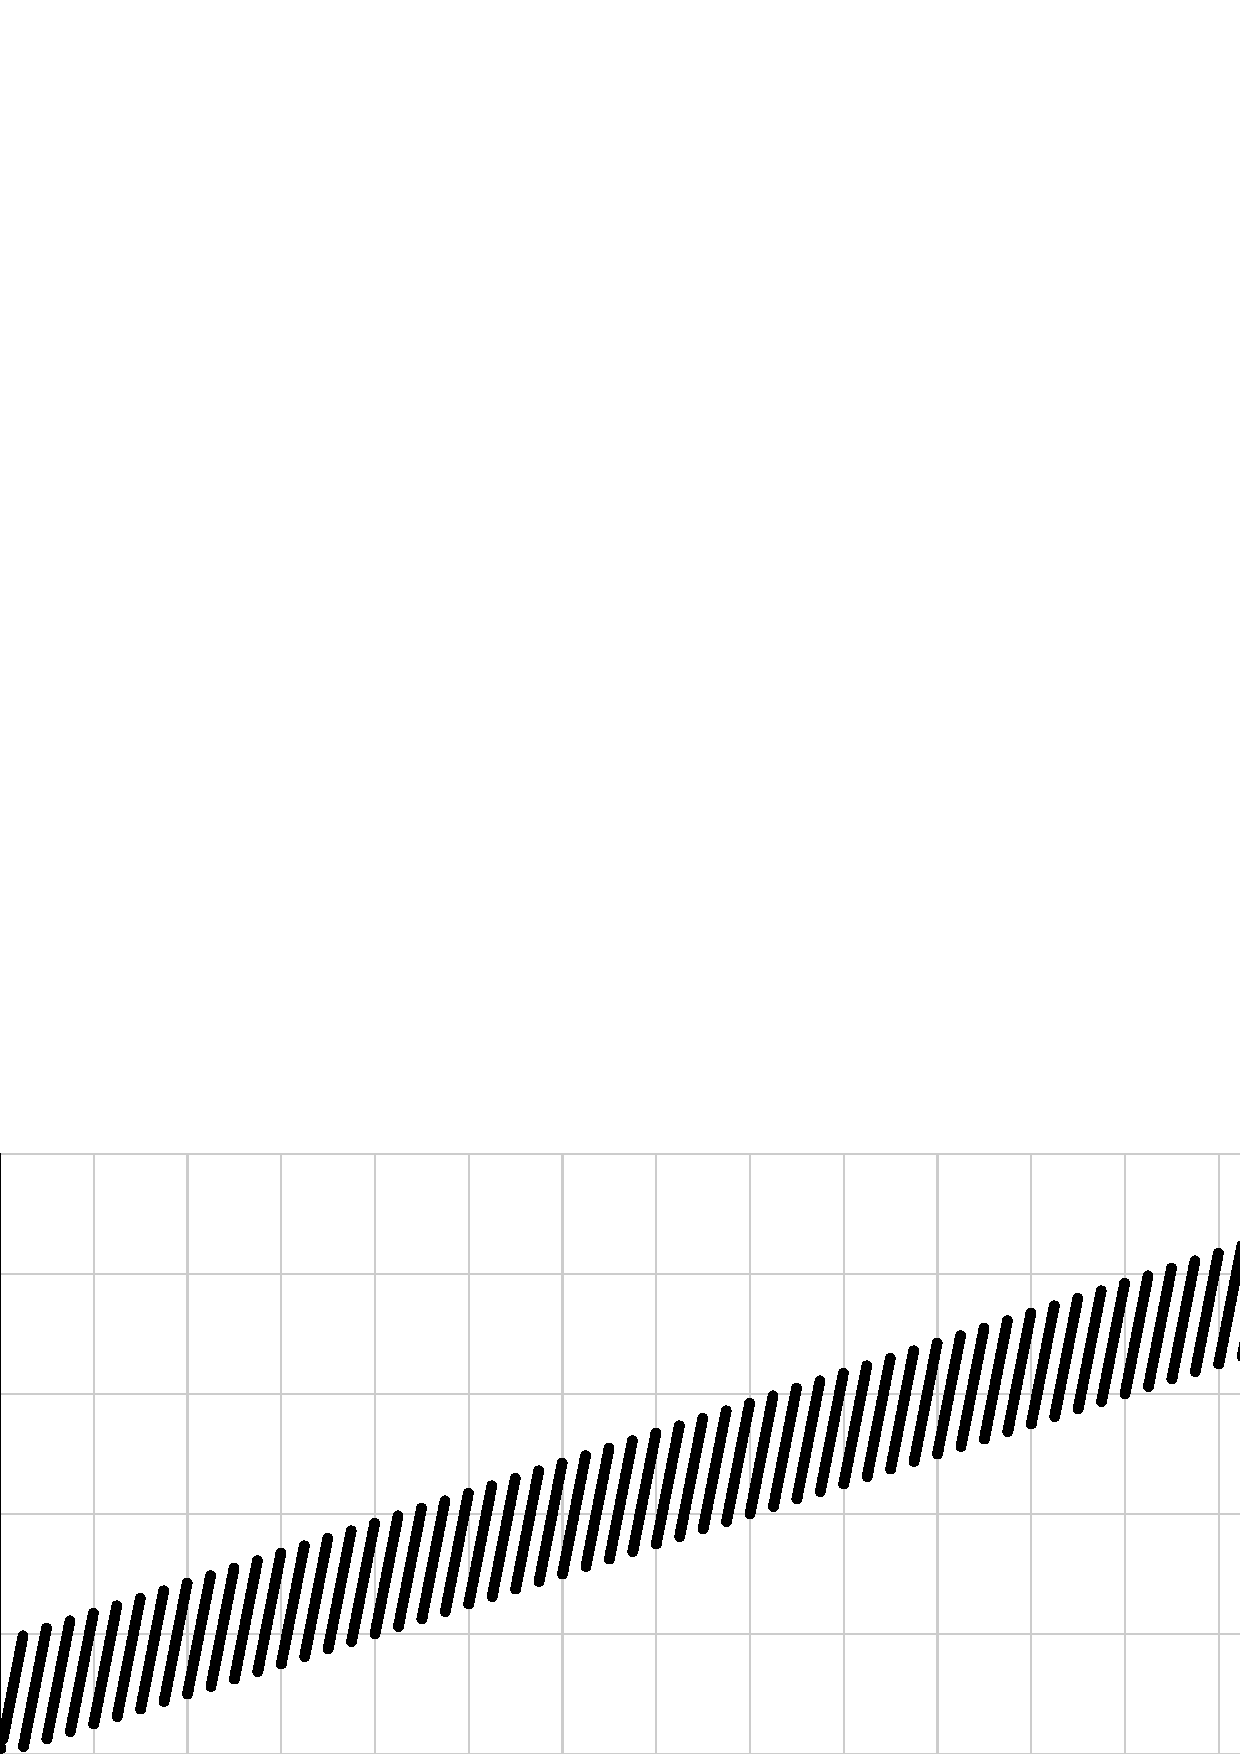
\includegraphics[width=\columnwidth]{figures/movsb.pdf}
\caption{On Pentium~D, the retired loads event shows unusual
       behavior with {\tt rep movs} string instructions.
       The observed count is related to 64-byte chunks being moved
       with individual moves for the remainder:
        $(floor(reps/64)*4)+(reps\%64)$.}
\label{figure:movsb}
\end{figure}

The Pentium~D event has complicated overcount, likely because
it is recording microcoded loads and not architectural loads.
Unlike other x86 processors, software
prefetches {\em are not} counted as loads and page faults 
count as five loads total.
Pop of a segment (fs/gs), {\tt movdqu} (load),
{\tt lddqu}, {\tt movupd} (load), and {\tt fldt} all count
as two loads instead of one. {\tt fldenv} counts as seven loads,
{\tt frstor} counts as 23 loads, and {\tt fxrstor} counts as 26.
The {\tt movups} (store) instruction counts as a load.
The {\tt fstps} instruction  counts as two (not zero) loads.

Unlike the other x86 load events that treat a rep-prefixed string
instruction as a single atomic instruction, on Pentium~D the
loads are counted separately, sometimes at a
cache-line granularity.  The {\tt rep lods} and {\tt rep scas} 
instructions count  each repeated load individually.  
The {\tt rep movs} instructions
performs moves in blocks of 64-bytes, then goes one-by-one
for the remainder (see \figurename~\ref{figure:movsb}).
The {\tt rep cmps} instruction counts each compare instruction
as two loads.

The SandyBridge load event measures load $\mu$ops so it has
limitations similar to Pentium D.  
On IvyBridge the event name
for this event was changed to make its $\mu$op nature more obvious.

\paragraph{Retired Store Overcount}

On Core2 processors the retired store event 
was found by Olszewski et al.~\cite{olszewski+:asplos09} to be deterministic
with no overcount, and we have reproduced this result.
All other processors count hardware
interrupts and page faults with store events.

On Nehalem and Westmere processors the {\tt cpuid}, {\tt sfence}, 
and {\tt mfence} instructions all count as stores (these are all
serializing instructions).  {\tt clflush} also counts as a store.

As with retired loads, the Pentium~D processor has elaborate
retired store behavior that likely exposes internal microcode
behavior.  As with Nehalem, the {\tt cpuid}, {\tt sfence}, {\tt mfence} 
and {\tt clflush} instructions count as a stores.
The {\tt enter} instruction counts an extra store for each nested stack frame.
The {\tt fbstp}, {\tt fstps}, {\tt fstpt}, {\tt movups} (store),
{\tt movupd} (store), {\tt movdqu} (store), and {\tt maskmovdqu} 
instructions counts as two stores.  The {\tt fstenv} instruction counts as 
seven stores, {\tt fsave} as 23 and {\tt fxsave} as 25.
The {\tt rep stos} string instruction counts stores 
in 16B blocks (unless storing backwards in memory).
The {\tt rep movs} instruction counts stores in 16B blocks.

The SandyBridge and IvyBridge store events measure $\mu$ops 
and have similar limitations to Pentium~D.

\subsubsection{Other Events}

Tables~\ref{table:results_uops}~and~\ref{table:results_fp} show results
from other events that we investigated as possibly being useful
deterministic events, but found to have too much microarchitectural
variation.  Total events are show to give a feel for the variation,
for comparison the dynamic total retired event count is
226,990,030.  The values shown are the average of ten runs, with
the plus/minus value indicating the maximum distance from the average.

\paragraph{Retired $\mu$ops}
Despite the ``retired'' modifier in the event name, 
$\mu$op behavior is nondeterministic as well as implementation
specific and cannot be relied on when comparing different machines.
The values are almost two orders of magnitude higher than the 
total instruction count; this is skewed by the fact that repeated
string instructions are only counted once by the retired instruction
event but counted individually by the $\mu$op event.

\paragraph{Multiplies and Divides}
Table~\ref{table:results_uops} also shows the numbers of 
multiplies and divides for each processor.  
Some of these counts are speculative or else count $\mu$ops; 
the documentation for the counters is not always clear.  
The implementation of these events varies from model to model;
some count integer only, some also count floating point and SSE, and some count
multiple times for one instruction.  
On Core2 {\tt divq} (64-bit divide) instructions also count as a multiply, 
and {\tt mulq} (64-bit multiplies) count twice.

On Atom and Bobcat processors the events are deterministic, but
these instructions are rare enough in most code that they
would likely not be useful in practice.

\paragraph{Floating Point and SSE}
Table~\ref{table:results_fp} shows results for various floating point,
MMX and SSE events.  Some of these events appear 
to be deterministic,
most notably the events on the AMD machines.  Unfortunately these events
are hard to predict via code inspection.  Some events are retired,
some speculative; some count retired instructions, some count retired
$\mu$ops.  Some count only math instructions, some count any sort
of instruction where floating point is involved.  Comparisons
between machines will not work due to these variations, and 
these events would not be useful for obtaining deterministic counts 
on integer-only benchmarks. 

\subsection{Other Architectures}

In addition to the x86\_64 architecture, we investigate other 
architectures to see 
if they have similar limitations with regard to determinism.

Creating a detailed microbenchmark like the one used on x86\_64
is a long and tedious process, and
we do not currently have sufficient resources to 
do this for every architecture.  
Instead we use the {\tt ll} assembly benchmark~\cite{weaver+:iccd09}
modified to repeat 10,000 times.  
This is not as comprehensive 
as the x86\_64 test (it does not test every possible opcode so 
may miss issues with overcount), 
but should catch any obvious determinism issues (such
as hardware interrupts being counted).

{\bf ARM}
We count retired instructions on ARM Cortex-A8 and Cortex-A9 processors.  
Unfortunately the performance counters on this architecture
cannot select only user-space events; kernel events are always counted too, 
which makes all of the available events non-deterministic.

{\bf IA64}
On Merced {\tt STORES\_RETIRED}, {\tt LOADS\_RETIRED}, and 
{\tt IA64\_INST\_RETIRED} appear to be deterministic.

{\bf POWER}
On a POWER6 system we find {\tt instructions:u} to be 
deterministic, but {\tt branches:u} suffers from
overcount.

{\bf SPARC}
Finally, on a SPARC Niagara T-1 system we find that the {\tt INSTR\_CNT} 
event is deterministic.
